\subsection{Lösungsansatz Task II}


\begin{frame}{Lösungsansatz Task II}
$\textbf{Idee}$: Prädiktionsmodell für Link Lifetime mit Einfluss des RSRP der verbunden sowie der Nachbarzellen \\
$\rightarrow$ Datentransformation nötig
	\begin{itemize}
		\item Anpassen der RSRP Messwerte in "Cells" an RSRP Werte in "Context"
		\item Cell Id $\rightarrow$ eNodeB 
		\item eNodeB Wechsel $\rightarrow$ Response Variable Link Lifetime
	\end{itemize} 

\quad\\

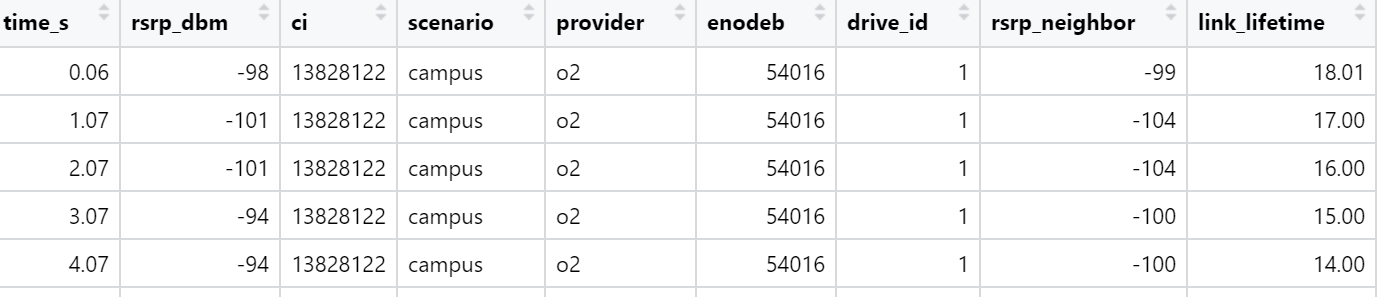
\includegraphics[width = 11cm]{table}
\end{frame}

\begin{frame}{Prädiktionsmodell Task II}
	\begin{itemize}
		\item Anwendung des Prädiktionsmodells XGBoost um Link Lifetime vorherzusagen 
		\item Validierung analog zu Task I mit Zeitreihenkreuzvalidierung
	\end{itemize}
\end{frame}